\section{Test Program}

Following is the supplied test program decoded from hexadecimal to assembly:

\begin{verbatim}
00: lw r1, 1(r0)    -- Data = 2
01: lw r1, 2(r0)    -- Data = 10
02: lw r1, 2(r0)    -- Data = 10
03: add r3, r1, r2
04: sw r3, 5(r0)
05: beq r0, r0, 2    -- Destination = 7
06: sw r3, 3(r0)
07: sw r3, 4(r0)
08: sw r3, 6(r0)
09: sw r3, 7(r0)
10: lui r3, 6
11: sw r3, 8(r0)
12: add r3, r1, r3
13: sw r3, 9(r0)
14: beq r0, r0, -3    -- Destination = 11
15: sw r3, 10(r0)
\end{verbatim}

\section{Simulation}

The execution of the first three instructions can be seen in figure \ref{fig:sim1}. As expected, these load word instructions makes use an extra stall cycle. The figure shows that data is loaded correctly from memory into the \emph{reg_write_data} signal, and that the register file is updated at the following clock cycle. Note that the register contents is too big to display in the figure, but the data is stored correctly. Since instruction 2 is indentical to instruction 1, nothing happens except for state traversal and incementation of the program counter.

\begin{figure}[ht]
    \centering
    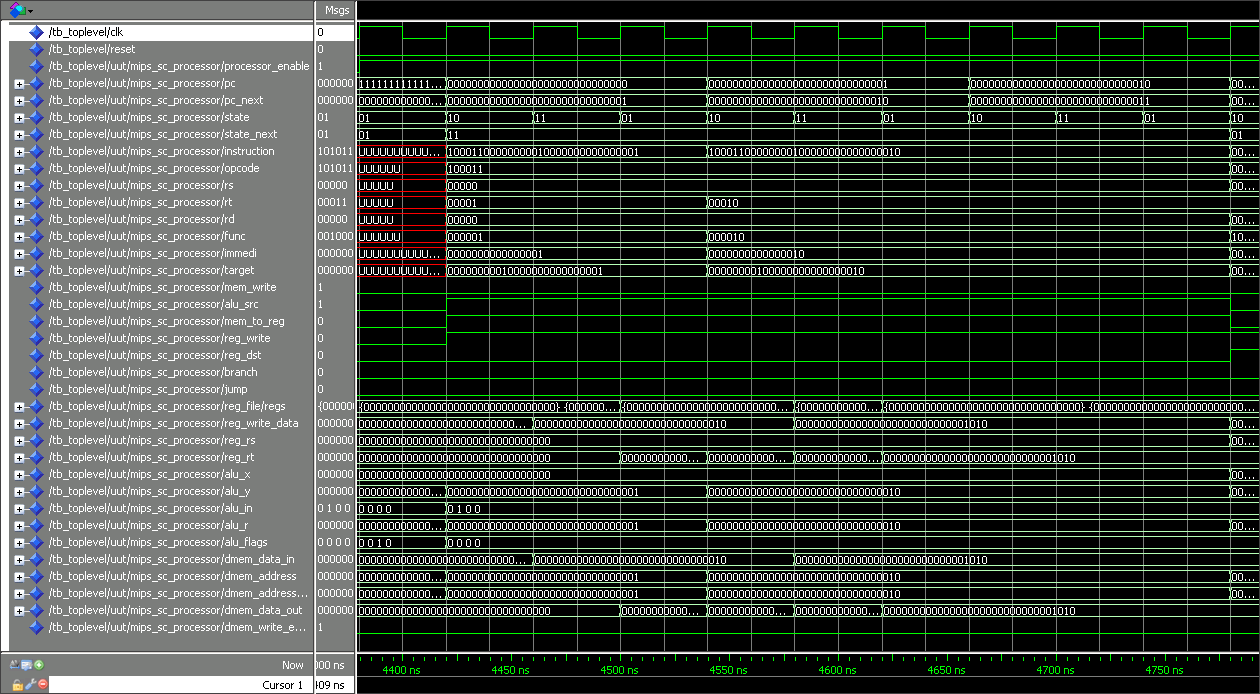
\includegraphics[scale=0.3]{figures/sim1.png}
    \caption{\label{fig:sim1}Simulation Part 1 - Instruction 0,1,2}
\end{figure}

Next, the action starts in figure \ref{fig:sim2}. First up is the add instruction, where the data from the load instructions are added together. The result can be seen in the signal \emph{alu_r}, and is written to registry 3 as specified by the signal \emph{rd}. Then the result is stored to the memory at address 5, which can be seen is successful as the signal \emph{dmem_data_in}, which is the data coming in to the processor from the data memory, reflects the change. Next the branch instruction can be seen asserting that zero is indeed equal to zero, and branches two instructions ahead to instruction 7, which stores register 3 to address 4.

\begin{figure}[ht]
    \centering
    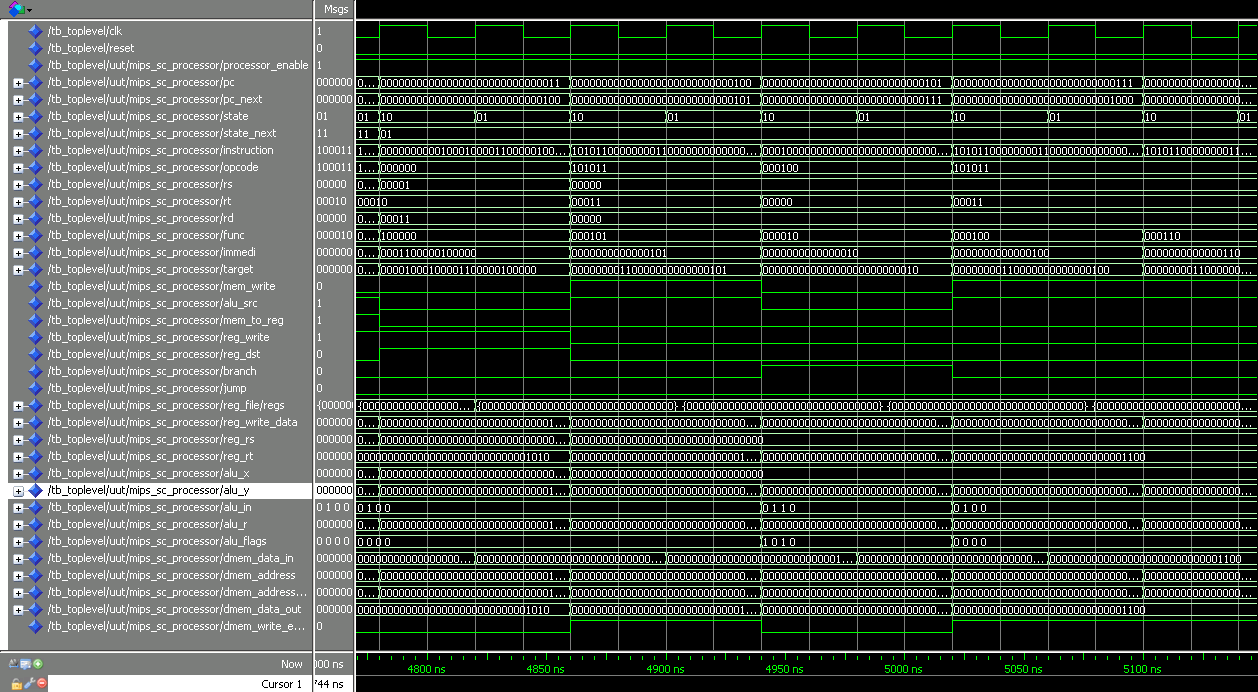
\includegraphics[scale=0.3]{figures/sim2.png}
    \caption{\label{fig:sim2}Simulation Part 2 - Instuction 3,4,5,7}
\end{figure}

In figure \ref{fig:sim3}, it can be seen that register 3 is also stored to address 6 and 7, before the load upper immediate function replaces the contents of register 3 by $6 << 16$, as seen in the signal \emph{reg_write_data}. Finally the result is stored to memory address 8.

\begin{figure}[ht]
    \centering
    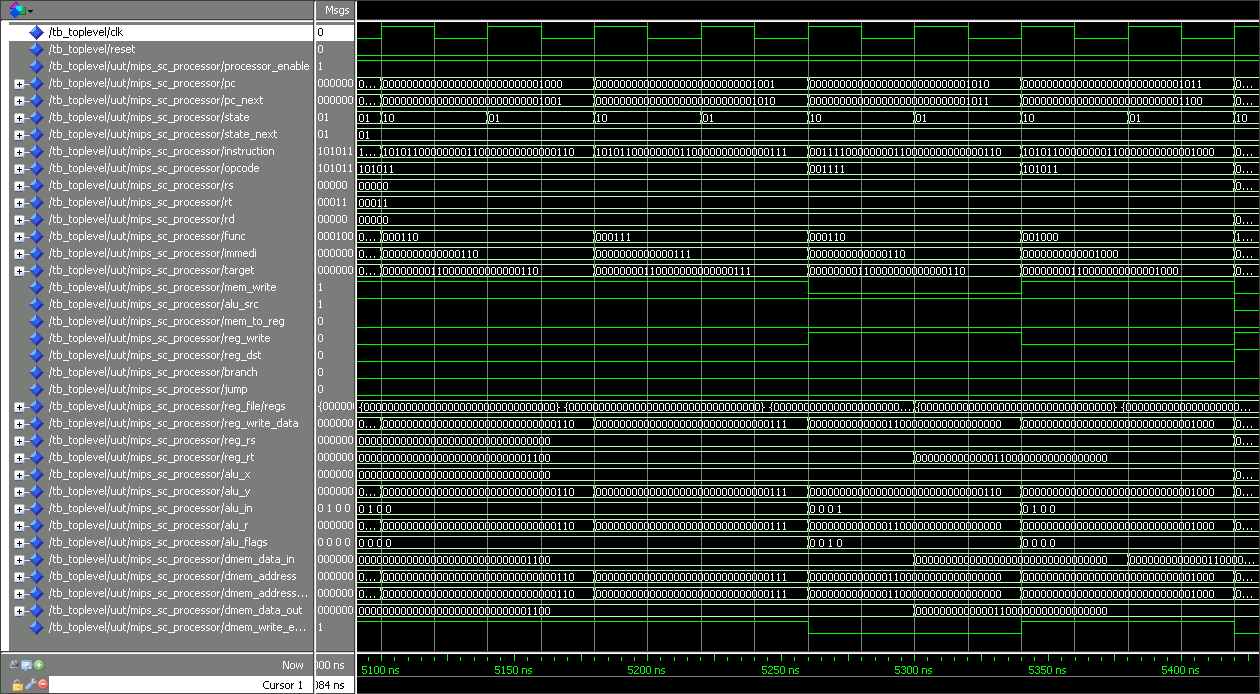
\includegraphics[scale=0.3]{figures/sim3.png}
    \caption{\label{fig:sim3}Simulation Part 3 - Instruction 8,9,10,11}
\end{figure}

Things are finished off in figure \ref{fig:sim4} where register 3 is set to register 3 added by register 1 before the result is also stored to the memory at address 9. Afterwards, the branch instruction once again asserts that zero is indeed zero, and jumps to instruction 11, doomed to repeat the same loop for all eternity, slowly increasing the contents of register 3.

\begin{figure}[ht]
    \centering
    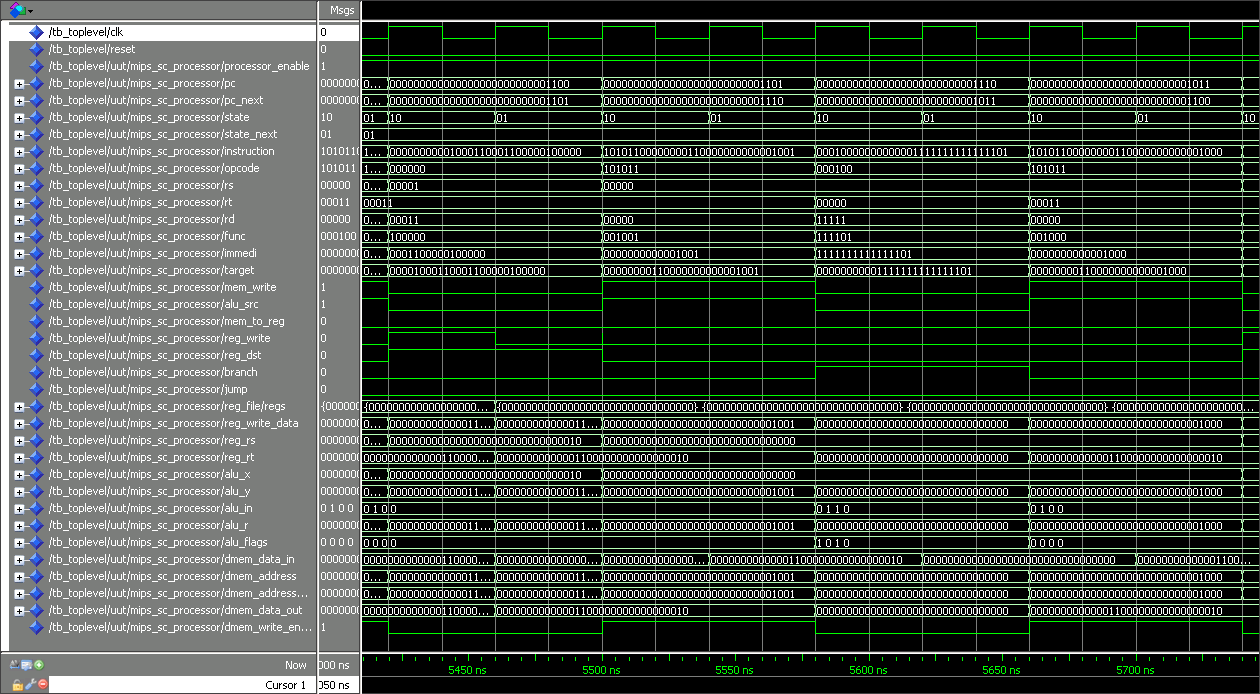
\includegraphics[scale=0.3]{figures/sim4.png}
    \caption{\label{fig:sim4}Simulation Part 4 - Instruction 12,13,14,11}
\end{figure}

TODO: Source
http://www.mrc.uidaho.edu/mrc/people/jff/digital/MIPSir.html
